\documentclass[a4paper, 10pt]{article}
\usepackage[utf8]{inputenc}
\usepackage[spanish] {babel}
\usepackage{amsfonts}
\usepackage{amssymb}
\title{Trabajo Practico 2}
\usepackage{tpalgo3}
\usepackage{caratula}
\usepackage{amssymb}
\usepackage[pdftex]{graphicx}
\usepackage{hyperref}


\setlength{\leftmargin}{10cm}
\setlength{\rightmargin}{10cm}
\setlength{\oddsidemargin}{-1cm}
\setlength{\evensidemargin}{-1cm}
\setlength{\topmargin}{-1cm}
\setlength{\textwidth}{18cm}
\setlength{\textheight}{25cm}

\usepackage{fancyhdr}
\pagestyle{fancy}
\fancyhf{}
\fancyhead [L]{\scriptsize Trabajo Práctico N$^{\circ}$2}
\fancyhead [R]{\scriptsize Aronson, Nahabedian, Ravasi}%1{20pt}
\fancyfoot[C]{\thepage}
\renewcommand{\footrulewidth}{0.4pt}

\begin{document}
\materia{Algoritmos y Estructuras de Datos III}
\submateria{Segundo Cuatrimestre de 2010}
\titulo{Trabajo Practico N$^{\circ}$2}
\grupo{Grupo 14}
\integrante{Aronson Alex}{443/08}{aronsonalex@gmail.com}
\integrante{Nahabedian Leandro Ezequiel}{250/08}{leanahabedian@hotmail.com}
\integrante{Ravasi Nicolás}{53/08}{nravasi@gmail.com}
\maketitle
\newpage

\tableofcontents
\newpage


\section{Ejercicio 1}

\subsection{Archivos}

En la carpeta $1$-$ej$ se puede encontrar
\begin{itemize}
\item $1$-$ej.cpp$: Algoritmo que resuelve el problema
\item $timer.cpp$: Usado para contar la cantidad de operaciones
\item $rangen.cpp$: Generador de inputs al azar
\item $pruebas.txt$ Casos borde usados para demostrar la correctitud
\item $input.txt$: Algunos casos que probamos a lo largo de la programación
\item $Makefile$

\end{itemize}

\subsection{Enunciado}

Se recibe una serie de cajas con las cuales se armará una única pila. Ante cada una de ellas se
puede tomar una de dos 
acciones, o se pone encima de la caja superior de la pila existente (inicialmente vacía), o se la
descarta totalmente. Cada
caja tiene un peso y una máxima carga soportada. La suma de los pesos de todas las cajas que están
encima de una caja
dada no puede superar su máxima carga soportada. Se debe calcular la máxima cantidad de cajas que es
posible apilar.


\subsection{Breve descripción del algoritmo}

Este problema decidimos resolverlo usando la técnica algorítmica de la programación dinámica. La idea de nuestro algoritmo es primero generar una matriz cuadrada de tamaño igual a la cantidad de cajas. Las filas van a representar las cajas vistas, y las columnas la cantidad de cajas descartadas. Al ver una por una las cajas, vamos a evaluar las diferentes posibilidades que surgen de tomar o descartar la caja en cuestión, manteniendo como valor de la matriz la capacidad máxima que soporta la pila para tal cantidad de cajas vistas y descartadas. Entonces, una vez vistas todas las cajas, el valor válido que encontremos más a la izquierda va a ser el máximo posible, sólo basta con encontrar dicho valor para poder dar el resultado\\

\nuevoAlgo{Algoritmo 1}{apilarCajas($cajas$ : $vector<caja>$, $n$ : $Nat$) $\rightarrow$ $res$ : $Nat$.
Devuelve la máxima cantidad de pilas que pueden ser apiladas, de acuerdo a las capacidades y los pesos dados.} \\

\begin{tabular}{rp{17cm}}
1: & apilarCajas ($cajas$ : $vector<caja>$)\ \{\vspace{0,1cm} \\ 
2: & \hspace{0,5cm}   capacidadesMaximas : Matriz$<$Nat$>$ $\gets$ NuevaMatriz($n$ x $n$, 0) \vspace{0,1cm} \\ 
3: & \hspace{0,5cm}   capacidadesMaximas$[0][0]$ = cajas.prim.capacidad\vspace{0,1cm} \\ 
4: & \hspace{0,5cm}   $\forall i \in$ $[0,cajas.tam)$\{\vspace{0,1cm} \\ 
5: & \hspace{1cm}	     $x$ = $i$\vspace{0,1cm} \\ 
6: & \hspace{1cm}	     $\forall$ j $\in$ $[0,i)$\vspace{0,1cm} \\ 
7: & \hspace{1.5cm}	     decidirSiApilar(capacidadesMaximas$[x][j]$)\vspace{0,1cm} \\ 
8: & \hspace{1.5cm}		 $x--$\vspace{0,1cm} \\ 
9: & \hspace{1cm}	  \}\vspace{0,1cm} \\ 
10: & \hspace{0,5cm}	  \}\vspace{0,1cm} \\ 
11: & \hspace{0,5cm}   x = cajas.tam-1\{\vspace{0,1cm} \\ 
12: & \hspace{0,5cm}   $\forall i \in$ $[0,cajas.tam)$\{\vspace{0,1cm} \\ 
13: & \hspace{1cm}	     \iif capacidadesMaximas$[x][i] > $-1 \vspace{0,1cm} \\ 
14: & \hspace{1.5cm}	     devolver x+1 \vspace{0,1cm} \\ 
15: & \hspace{1cm}	     $x--$\vspace{0,1cm} \\ 
16: & \}\\ \vspace{0,1cm} \\ 
\end{tabular}


La función decidirSiApilar mira tanto hacia su izquierda como hacia arriba de la posición en la que está parada, si la capacidad resultante de tomar el mínimo de la capacidad de la caja actual y la que sale de apilar la caja actual con la capacidad que la que viene dada a izquierda (siempre y cuando se pueda apilar) es mayor que la que está arriba, coloca la misma, sino, coloca la misma cantidad que tenía arriba suyo. En caso de estar en la fila 0, compara la capacidad que viene dada a izquierda con la capacidad de la caja actual que quiere apilar (porque la capacidad del piso es infinita, entonces no importa el peso de dicha caja). En caso de estar en la columna 0, se fija al colocar la caja no excede el peso máximo soportado, si puede, resta el peso, si no, coloca -1 para significar que esa vía no es posible. 


\subsection{Correctitud}


Sea un vector de cajas cualquiera, queremos demostrar que la matriz en una iteración k-ésima tiene la mayor capacidad que se puede obtener si se descartan de 0 a k-1 cajas. Se puede ver que si esto es verdad, al terminar de iterar sobre las cajas, se va a tener todas las capacidades resultantes descartando de 0 a n cajas; lo único que queda ver es cuál es el primer resultado en la matriz que tiene una capacidad válida (o sea, mayor o igual a 0), recorriendo en diagonal desde la esquina inferior izquierda hasta la superior derecha, la fila del primer resultado positivo denota la cantidad de cajas apiladas menos uno.

Debemos ver que los resultados puestos en la matriz son efectivamente los mejores en dicho momento, para esto primero veamos que dado una cantidad de cajas, siempre va a haber un mejor resultado (dado por la capacidad máxima soportada por la pila) para cada cantidad de cajas apiladas, ya sea apilar todas, todas excepto una, y así hasta llegar a apilar una sola caja y descartar todas las otras que se recibieron hasta ese momento. Para el caso de apilar todas, nuestro algoritmo lo hace, si puede, en caso de descartar todas menos una, nuestro algoritmo siempre elije apilar la de mayor capacidad. En el caso medio, digamos que habiendo visto $i$ ($0 < i < n$) cajas descartamos $j$ ($0 < j < i$); llegamos a la posición ($i$,$j$), en ($i-1$,$j$) tenemos la capacidad obtenida si se descartan $j$ cajas para $i-1$ cajas vistas; en ($i$,$j-1$), la capacidad si se descartan $j-1$ cajas para $i-1$ cajas vistas. Puede verse que tanto si apilamos la caja actual para el primer caso como si la descartamos para el segundo, vamos a tener una situación con $i$ cajas vistas y $j$ descartadas; podemos ver que uno de esos dos casos da una capacidad total mejor (o igual) que el otro, para esto hay que ver si al apilar la caja, tomando el mínimo entre la resta de capacidad que venía dada en ($i-1$, $j$) y el peso de la caja actual, y la capacidad de dicha caja; si comparamos esto con la capacidad en ($i$,$j-1$), el que sea mayor va a dar cuál es la mejor forma de apilar para $i$ cajas y $j$ descartadas.

Con esto probamos que dada una instancia, esta se setea correctamente. La matriz la construimos de $n$ x $n$, con $n$ la cantidad de cajas, las filas indican las cajas apiladas (teniendo en cuenta que se empieza desde 0) y las columnas la cantidad de cajas descartadas. Como la matriz la recorremos en diagonal, podemos asegurar que tomamos todos los casos y que estos son válidos, puesto que primero vamos a considerar $n$ apiladas y 0 descartadas, luego $n-1$ apiladas y una descartada, y así sucesivamente hasta llegar a descartar a todas.


\subsection{Complejidad}

La complejidad algorítmica de este problema no necesita de mucho análisis. Lo que realizamos efectivamente es primero la creación de una matriz inicializada en $-1$ de tamaño $NxN$. Como debo asignar un valor para cada posición esto cuesta $O(n*n) = O(n^2)$.

Luego recorremos la misma matriz nuevamente, esta vez en otro orden. La orientación de como recorremos es en diagonal, completando primero los valores de la parte superior izquierda de la matriz. Es decir, completaremos el triangulo formado por las posiciones $(0,0),(n,0)$ y $(0,n)$, recorriendo las sucesivas diagonales desde la parte inferior derecha hacia la superior izquierda. En cada posición de la matriz, realizamos ciertas operaciones basadas en lecturas de las celdas adyacentes, sumas, restas y utilizar la función $max()$\footnotemark o $min()$\footnotemark de la stl. De acuerdo a la implementación de estas funciones, solo realizan funciones constantes.

Finalmente, en esta sección se ejecuta $n*n$ veces operaciones constantes. Por lo tanto, la complejidad de cargar los valores en la matriz es del orden de $O(n^2)$.

Lo ultimo que realiza nuestro algoritmo es recorrer la diagonal $(n,0)$ hasta $(0,n)$ y tomar el primer valor que no sea $-1$, este ciclo hace una recorrida de $n$ celdas, únicamente leyendo si es o no distinto de $-1$ dando como complejidad total la siguiente cuenta:

\begin{center}
$O(n^2) + O(n^2) + O(n) \in O(n^2)$
\end{center}

Como el enunciado pedía que la complejidad fuera menor estricta que $n^3$, nuestra cota cumple con lo pedido ya que $n^2 < n^3$ para todo $n > 1$.

\footnotetext[1]{\url{http://www.cplusplus.com/reference/algorithm/max/}}
\footnotetext[2]{\url{http://www.cplusplus.com/reference/algorithm/min/}}

\newpage 

\subsection{Tablas y Gráficos}

Para este ejercicio notamos que no existe un peor caso, puesto que en todos los casos se debe generar la matriz completa (en realidad, la mitad de la matriz $n$ x $n$); sin importar de qué valores tengan las capacidades y pesos de las cajas pasadas por parámetro. Es importante recalcar que si las cajas nunca se pueden apilar, al recorrer en diagonal la matriz luego de haberla generado buscando el primer valor que no es igual a -1 va a haber que recorrer toda la diagonal y por ende las operaciones aumentarán, pero no lo harán demasiado porque la diferencia es del orden de $O(n)$, y el algoritmo tiene complejidad $O(n^{2})$, entonces la diferencia es relativamente menor.\\

A continuación presentamos la tabla y el gráfico obtenidos de medir la cantidad de operaciones que se efectúan con $timer.cpp$ para diferentes cantidades de cajas que fueron generadas con $rangen.cpp$; estos datos contrastados con los teóricos que demuestran que nuestras mediciones se mantienen siempre por debajo de la curva $c * n^{2}$, con $c$ tomando el valor de 5.

 
\begin{center}
\begin{tabular}{|c|c|c|}
\hline
Cantidad de cajas & Cantidad experimental de operaciones & Caso Teórico: $5 * n^{2}$\\
\hline
10 & 332 & 500\\
\hline
20 & 1,265 & 2,000\\
\hline
30 & 	2,799	 & 4,500\\
\hline
40	 & 4,936	 & 8,000\\
\hline
50 & 	7,663	 & 12,500\\
\hline
75 & 	17,153	 & 28,125\\
\hline
100	 & 30,366	 & 50,000\\
\hline
150	 & 68,056	 & 112,500\\
\hline
200	 & 120,748 & 	200,000\\
\hline
300 & 	271,139	 & 450,000\\
\hline
400	 & 481,537	 & 800,000\\
\hline
600	 & 1,082,295 & 	1,800,000\\
\hline
800	 & 1,923,110	 & 3,200,000\\
\hline
1,000 & 	3,003,895	 & 5,000,000\\
\hline
\end{tabular}
\end{center} \vspace{0,15cm}


\begin{center}
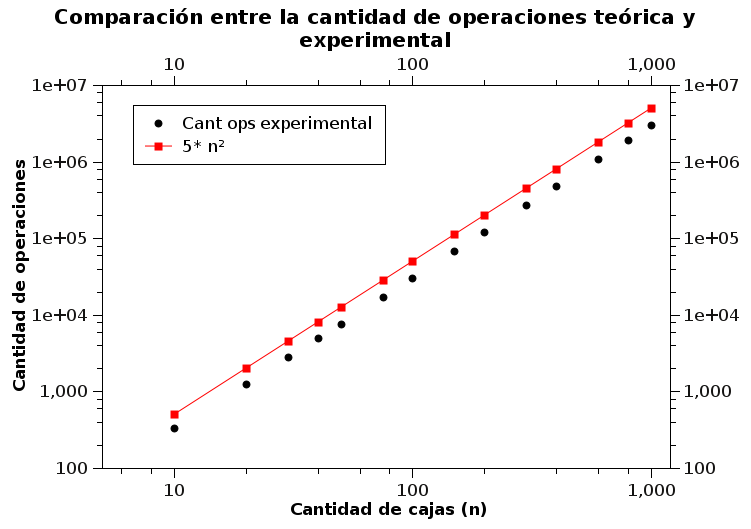
\includegraphics[scale=0.60]{graficos/1-1.png} \\
\scriptsize{\textsf{\textbf{Gr\'afico 1.1}}}  \\
\end{center}

\newpage
\subsection{Casos de Prueba}

A lo largo de las pruebas de este ejercicio hemos probado múltiples casos de prueba, para poder verificar que efectivamente nuestro algoritmo cumpla con todas
las especificaciones dadas.
Evaluamos que para este problema había un conjunto de tests en el que podíamos encontrar fallas al momento de correr el programa.
Los casos evaluados fueron los siguientes (pueden encontrarse en $pruebas.txt$)
\begin{itemize}
\item Un caso borde en el que todas las cajas dadas por parámetro podían ser apiladas. Esto se puede generar poniendo cajas de peso mínimo con distintos valores de soporte de las mismas.

\begin{verbatim}
1 10
1 9
1 8
1 7
1 6
\end{verbatim}

Este caso demuestra que el algoritmo soporta apilar una después de otra cuando es posible, en este caso como todas se pueden apilar sin necesidad de descartar ninguna, se apilan todas

\item Otro caso evaluado fue aquel en que solo podía apilarse una sola caja. Esto lo generamos poniendo una caja que soporte un valor imposible de alcanzar por las cajas restantes ya que le colocamos un peso mayor a todas, y así sucesivamente para el resto.

\begin{verbatim}
1 1
2 2
3 3
4 4
5 5
\end{verbatim}

Este caso demuestra que el algoritmo no apila cuando no puede, y se queda con una sola caja si es lo único que puede hacer


\item Un tercer caso evaluado es aquel en el que la mejor opción es descartar la primer caja porque esto causará que se puedan apilar más cajas.

\begin{verbatim}
4 5
6 10
4 6
4 2
2 1
\end{verbatim}

Aquí se puede ver que si se apila la primera sólo se puede apilar una caja más, mientras que si se la descarta y se apila la segunda, se pueden apilar cuatro, esto demuestra que nuestro algoritmo descarta bien las cajas cuando debe y sólo apila cuando le es conveniente

\item Un último caso en que sólo tiene una caja
\begin{verbatim}
48 21
\end{verbatim}

Este caso sirve para demostrar que el primer elemento de la matriz se genera correctamente y además el algoritmo se comporta bien aún cuando no hay iteración que hacer

\end{itemize}

\newpage
\section{Ejercicio 2}

\subsection{Archivos}

En la carpeta $2$-$ej$ se puede encontrar
\begin{itemize}
\item $2$-$ej.cpp$: Algoritmo que resuelve el problema
\item $timer.cpp$: Usado para contar la cantidad de operaciones
\item $pruebas.txt$: Casos borde usados para demostrar la correctitud
\item $testcant.txt$: Tests que varían la cantidad de palabras usados para evaluar complejidad
\item $testquer.txt$: Tests que varían la cantidad de queries usados para evaluar complejidad
\item $testlong.txt$: Tests que varían la longitud de las palabras usados para evaluar complejidad
\item $Makefile$

\end{itemize}

\subsection{Enunciado}

Se tiene el juego de transformación de palabras. El juego consiste en dadas una palabra de inicio y otra de fin, ambas del
 mismo tamaño, y un diccionario de palabras, determinar cuál es la mínima cantidad de reemplazos de una letra necesarios
para pasar de la palabra origen a la destino, generando palabras válidas del diccionario en los pasos intermedios. Por
ejemplo la palabra "sol" se puede convertir en "mar" mediante la transformación "sol - sal - mal - mar".


\subsection{Breve descripción del algoritmo}

Para resolver este problema decidimos dividir la solución en dos partes, la primera parte modela un grafo con todas las palabras pasadas por parámetro en el diccionario, estas palabras las agregamos a un vector que les asigna un número de referencia, luego son agregadas con dicho número a un mapa que nos permitirá obtener su número de referencia rápidamente, esto lo hacemos para trabajar con ints que nos permiten indexar en arrays con facilidad y desligarnos de las palabras. Una vez referenciadas, debemos construir el grafo, este lo vamos a mantener en un vector de arrays, para cada palabra vamos a tener un array que nos va a indicar si está relacionada con cada una de las demás (relacionada significa que posee un carácter de diferencia a lo sumo).

Una vez hecho esto, podemos examinar las diferentes queries que nos llegan, para resolver esta parte del problema usaremos un BFS. Éste funcionará de la siguiente manera, para el nodo de inicio vamos a ver todos sus adyacentes y los vamos a marcar como nodos de nivel 1, luego para cada nodo de estos vamos a ver sus adyacentes y marcarlos como nivel 2 a menos que ya hubieran estado marcados, y así sucesivamente hasta dar con la palabra destino que estamos buscando.

A continuación presentamos el pseudocódigo pero solo del BFS.\\

\newpage
\nuevoAlgo{Algoritmo 2}{ReemplazosMinimos($diccionario$ : $dicc(palabra, adyacentes)$, $origen$ :
$palabra$, $destino$ : $palabra$) $\rightarrow$ $res$ : $Nat$. Donde $adyacentes$ es
$conj<palabra>$. Devuelve la mínima cantidad de reemplazos necesarios para pasar de la palabra
origen a la palabra destino.} \\

%\begin{}

\begin{tabular}{rp{17cm}}
1: & ReemplazosMinimos ($diccionario$ : $dicc(palabra, adyacentes)$, $origen$ : $palabra$, $destino$ : $palabra$)\{\\
2: & \hspace{0,5cm}   cola : queue(palabra, distancia) $\gets$ Vacia \vspace{0,1cm} \\ 
3: & \hspace{0,5cm}   marcados : vector(bool) $\gets$ NuevoVector(false) \{\vspace{0,1cm} \\ 
4: & \hspace{0,5cm}	  cola.push(origen, 0)\vspace{0,1cm} \\ 
5: & \hspace{0,5cm}	  marcados[origen] $\gets$ true\vspace{0,1cm} \\ 
6: & \hspace{0,5cm}	  \mientras (!cola.empty()) \{\vspace{0,1cm} \\ 
7: & \hspace{1cm}	    proximo : palabra $\gets$ proximo(cola)\vspace{0,1cm} \\ 
8: & \hspace{1cm}	    distancia : Nat $\gets$ $\pi_2$(proximo)\vspace{0,1cm} \\ 
9: & \hspace{1cm}       marcados[proximo] $\gets$ true\vspace{0,1cm} \\ 
10: & \hspace{1cm}	    $\forall$ v $\in$ diccionario.obtener($\pi_1$(proximo)) \{\vspace{0,1cm} \\ 
11: & \hspace{1,5cm}          \iif(noEstaMarcado(marcados, v))\vspace{0,1cm} \\ 
12: & \hspace{2cm}	             cola.push(v, distancia + 1)\vspace{0,1cm} \\ 
13: & \hspace{1,5cm}          \finif\vspace{0,1cm} \\ 
14: & \hspace{1cm}	    \}\vspace{0,1cm} \\ 
15: & \hspace{0,5cm}  devolver distancia \vspace{0,1cm} \\ 
16: & \}\\ \vspace{0,1cm} \\ 
\end{tabular}


La función $push()$ es la que esta implementada en la librería de $C++$


\subsection{Correctitud}

En este problema lo esencial es realizar un buen modelo que, una vez conseguido, basta con aplicarle un algoritmo conocido para llegar a la solución. El modelo utilizado se basa en que las palabras serán nodos en nuestro grafo y dos palabras (nodos) están unidas por un eje si y sólo si las palabras son iguales en longitud y difieren en exactamente una letra. Luego de modelar de esta forma el problema, utilizamos el algoritmo de BFS para conocer la distancia mínima desde una palabra a otra.\\

Para chequear cuando dos palabras son adyacentes, verificamos primero que tengan la misma longitud y luego recorremos ambas y verificamos cuantas coincidencias de letras hay, contemplando en cada comparación, la posición de las mismas. Como dos palabras son adyacentes cuando difieren en una letra, entonces pedimos que dicho contador sea igual a la longitud de una palabra - 1.

Luego como dos palabras (nodos) son adyacentes cuando difieren en una letra y su longitud es igual, en nuestro modelo, ir de un nodo a otro utilizando un eje se traduce a realizar un reemplazo de palabras. La idea con este modelo es que dado las dos palabras recibidas como parámetro viajemos a través de nodos y ejes hasta conseguir un camino mínimo desde la palabra origen hasta la palabra destino.

Ahora lo que deseamos es utilizar un algoritmo que recorra todo el grafo y nos de el camino mínimo desde el nodo origen hasta el nodo destino, y contando la cantidad de ejes que se necesitan recorrer para transformar la palabra origen en la palabra destino. Como atravesar un eje es reemplazar una letra por otro, la cantidad de ejes atravesados es igual a la cantidad de reemplazos necesarios. Si la cantidad de ejes es mínima, entonces la cantidad de reemplazos también lo es.\\

Luego, debemos probar porque el algoritmo de BFS consigue algún camino mínimo desde el nodo origen, hasta el nodo destino. Para esto veamos lo siguiente: BFS recorre todo el grafo pasando una única vez por cada nodo, empezando desde la raíz y marcándolos para no volverlos a pisar. Nosotros utilizamos como raíz al nodo origen y modificamos el algoritmo típico de BFS para que además de marcar los nodos, nos interesamos por saber cuan lejos esta este nodo desde el nodo raíz, es decir, desde el origen. Como el algoritmo de BFS recorre a los nodos por nivel, es decir, primero a todos los nodos de nivel 1. Cuando no hay mas nodos de nivel 1, es decir los nodos adyacentes a la raíz, empieza a recorrer los nodos de nivel 2, es decir los adyacentes a algún nodo de nivel 1.

Siguiendo así con el algoritmo, como hacemos BFS y el mismo nos asegura que marca todos los nodos y nosotros les ponemos a cada nodo su nivel correspondiente, estamos seguro que en algún momento llegaremos al nodo destino y lo marcaremos con el la distancia correcta hasta el origen. Recordemos que nuestro algoritmo si vuelve a pasar por un nodo ya marcado, como recorre los nodos por niveles, seguro que el nivel que quiere colocarle a ese nodo va a ser mayor que el que ya tenia.\\

Supongamos que el nodo destino esta a nivel $h$ y nuestro algoritmo le da nivel $p$  ($p \neq h$). Pero nuestro algoritmo pone 1 a los adyacentes de la raíz, 2 a los adyacentes de los nodos de nivel 1, y así sucesivamente. Por lo tanto hay algún camino de longitud $p$ desde el nodo raíz (origen) hasta el nodo destino, pues se ejecute $p$ veces la rutina de marcar adyacentes.

Pero si $p < h$ entonces no tenemos forma de atravesar $p$ ejes y llegar al nodo destino. Absurdo

Y si $p > h$ entonces marcamos al nodo destino dos veces. Como voy recorriendo todos los nodos de nivel 1, todos los de nivel 2, y así siguiendo, seguro que vamos a pasar por $h$, antes que por $p$ pero nuestro algoritmo una vez que marca, no vuelve a marcar. Absurdo

Finalmente BFS con su modificación funciona correctamente.






\subsection{Complejidad}

Para comenzar a resolver este ejercicio debemos determinar de que manera armaremos el grafo para poder en este aplicar la solución a través del algoritmo de BFS, estas complejidades son separadas y se van a sumar después para dar la definitiva.

Dicho esto, para construir el grafo tomamos todas las palabras y las colocamos en un vector. Así, luego asignamos a cada una un número dado por cómo están ordenadas y hacemos un mapa de referencias, esto lo hacemos porque después es más fácil hacer el BFS si las referencias son enteros, de manera que cada vez que preguntemos por una palabra podemos obtener la referencia en orden logarítmico y después no tener que preocuparnos por la misma. Para construir el diccionario, leemos las palabras de a una y las insertamos al mismo con su número de orden correspondiente, sabemos que el peso de insertar \footnotemark una palabra al diccionario es $log (n) * l$, siendo $n$ la cantidad de palabras y $l$ la longitud máxima que es lo que va acomparar en cada caso al pushear en el mapa; entonces generar el mapa de referencias cuesta $n * log (n) * l$.

Luego debemos generar los vectores de adyacencias, para esto va a haber que comparar todas las palabras contra todas, lo que nos causa un doble $for$ ya que vemos todas las palabras y las comparamos con todas las que están hacia adelante. Para determinar si son adyacentes, primero preguntamos si la longitud es la misma y luego si están relacionadas.

En esta función lo que hacemos es, asumiendo que un String es una cadena de tipo Char, es decir podemos preguntar a través de una variable i, una posición y así saber el valor de la letra. Tomando como parámetro, las palabras que tenemos en nuestro diccionario, a partir de dos palabras de misma longitud, recorremos letra a letra y así determinar si son o no adyacentes. Como esto lo hacemos por cada palabra de nuestro diccionario, asumiendo $l$ como la longitud máxima de una palabra que hay en el diccionario, y al tener que recorrer todo String como Array de Char, esta función tiene entonces un costo de orden $l$.

Si están relacionadas, simplemente debemos obtener las referencias en el mapa con costo logarítimico y agregarlos a los vectores de adyacencia correspondiente en tiempo constante, por lo tanto, esta parte tiene costo en total $n^{2} * log (n) * l$

Una vez formado el grafo con todas las adyacencias previamente calculadas, pasamos a resolver la esencia del problema que es determinar las distancias de todos los pares de palabras obtenidos por parámetro tal como lo marca la consigna. Para lograr esto, decidimos que a medida que vamos obteniendo un par de palabras para consultar la distancia, llamamos a la función Search que es la encargada de resolver el ejercicio. Como esto lo hacemos por cada par de palabras que obtenemos, siendo m la cantidad de consultas, terminaremos llamando a la función Search en un total de m veces, esto tendrá una complejidad de orden m por cada llamada a la función que resuelve el problema.

En cada search, primero obtenemos en el mapa de referencias las posiciones en el array de las palabras que se piden, esto tiene costo $l * log (n)$ para cada una; una vez hecho esto iniciamos el BFS, primero creando una cola vacía y un vector de bool inicializado todo en false (2-3 en el pseudocódigo), para esto usamos el contenedor de la librería $C++$, llamado $queue$ y $vector$. El constructor de $queue$\footnotemark y el constructor de $vector$\footnotemark tienen complejidad constante. Luego, en 4 realizamos la operación $push()$\footnotemark de la librería de $C++$ esto tiene costo constante, marcando la posición inicial en el array (5). 

\footnotetext[3]{\url{http://www.cplusplus.com/reference/stl/map/insert/}}
\footnotetext[4]{\url{http://www.cplusplus.com/reference/stl/queue/queue/}}
\footnotetext[5]{\url{http://www.cplusplus.com/reference/stl/vector/vector/}}
\footnotetext[6]{\url{http://www.cplusplus.com/reference/stl/queue/push/}}


Una vez hecho esto, podemos iniciar el ciclo del BFS, esto lo va a hacer por cada elemento en la cola (6), en ésta puede entrar como mucho cada nodo una vez (sólo se pushean los marcados), por lo tanto el ciclo se va a ejecutar n veces en peor caso. Dentro del mismo, vemos (7-8) el próximo de la cola\footnotemark \footnotetext[7]{\url{http://www.cplusplus.com/reference/stl/queue/front/}}  y lo popeamos,\footnotemark \footnotetext[8]{\url{http://www.cplusplus.com/reference/stl/queue/pop/}} ambos en tiempo constante. Luego, tenemos un nuevo ciclo, en el que vamos a ver todos los adyacentes del mismo, si están marcados, los obviamos, si no, los agregamos a la cola; estas operaciones ya dijimos que eran constantes, en peor caso (el grafo completo), el nodo tiene n-1 adyacentes, por lo tanto el ciclo se ejecutará $n$ veces.




En total, se puede ver que el search tiene complejidad $O(n^{2} + l * log (n))$, y en total todos los search van a costar $O(m * n^{2} + l * log (n))$

En resumen, la complejidad total es la suma de la de crear el mapa, la de crear los vectores de adyacencias y la de hacer todos los search, o sea, \\
\begin{center}
$O(n * log (n) * l) + O (n^{2} * log (n) * l) + O(m * n^{2} + l * log (n) =  O (n^{2} * log (n) * m * l) < O(n^{2.5}*m*l)$
\end{center}

porque $O(log(n)) < O(\sqrt{n})$ 





\subsection{Tablas y Gráficos}

Para confeccionar los gráficos, usaremos nuevamente un archivo $timer.cpp$ el cual cuenta la cantidad de operaciones efectuadas para cada diccionario, con todos sus queries incluidos. Debido a la dificultad de hacer un generador random para este algoritmo, decidimos recurrir al testeo mediante casos hechos a mano. Como existen tres diferentes variables que afectan a la complejidad, haremos un testeo para cada una dejando fijas las otras dos, primero variaremos la longitud máxima de las palabras manteniendo constante la cantidad de queries y de palabras en el diccionario; luego alteraremos la cantidad de búsquedas dejando fijas la longitud y el tamaño del diccionario; por último, cambiaremos la cantidad de palabras dejando constante las queries y la longitud. En todos casos agregamos la curva teórica que resulta de aplicar la complejidad con los valores obtenidos

Para facilitar la creación de diferentes queries, los grafos resultantes de cada diccionario son siempre conexos.

\begin{center}
\begin{tabular}{|c|c|c|}
\hline
Longitud de palabra & Cant. de ops. para $n=10$ y $m=5$ & Curva teórica $n^{2}*log(n)*m*l$,$n=10$ y $m=5$\\
\hline
3	&	788 & 1,500\\
\hline
4	 & 978	 & 2,000\\
\hline
5 & 	1,214 & 	2,500\\
\hline
6 & 	1,500 & 	3,000\\
\hline
7 & 	1,458 & 	3,500\\
\hline
8	 & 1,670	 & 4,000\\
\hline
9 & 	1,955	 & 4,500\\
\hline
\end{tabular}
\end{center} \vspace{0,15cm}



\begin{center}
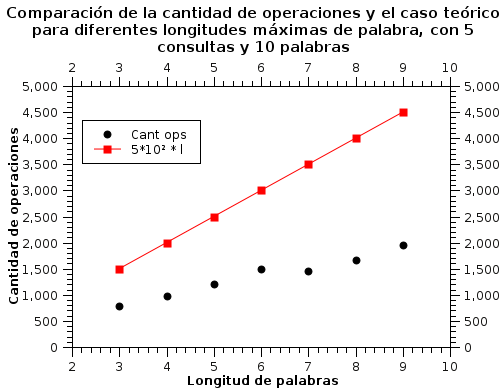
\includegraphics[scale=0.70]{graficos/2-1.png} \\
\scriptsize{\textsf{\textbf{Gr\'afico 2.1}}}  \\
\end{center}

\begin{center}
\begin{tabular}{|c|c|c|}
\hline
Queries & Cant. de ops. para $n=10$ y $l=9$ & Curva teórica $c*n^{2}*log(n)*m*l$, $c=2$, $n=10$ y $m=5$\\
\hline
1	& 1,654	& 1,800\\
\hline
2	& 1,720	& 3,600\\
\hline
3	& 	1,792	& 	5,400\\
\hline
4	& 	1,892	& 	7,200\\
\hline
5	& 	1,955	& 	9,000\\
\hline
6		& 2,034	& 	10,800\\
\hline
7		& 2,112		& 12,600\\
\hline
8	& 	2,185		& 14,400\\
\hline
9		& 2,354		& 16,200\\
\hline
10		& 2,417		& 18,000\\
\hline
\end{tabular}
\end{center} \vspace{0,15cm}



\begin{center}
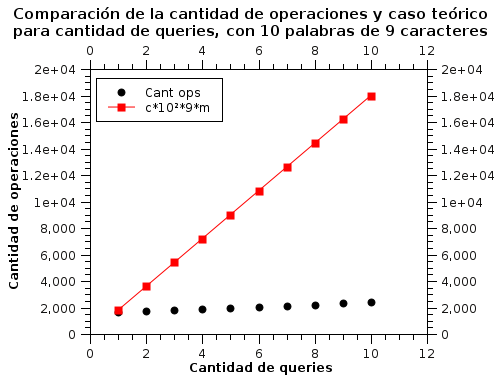
\includegraphics[scale=0.70]{graficos/2-2.png} \\
\scriptsize{\textsf{\textbf{Gr\'afico 2.2}}}  \\
\end{center}



\begin{center}
\begin{tabular}{|c|c|c|}
\hline
Tamaño del diccionario & Cant. de ops. para $m=5$ y $l=9$ & Curva teórica $n^{2}*log(n)*m*l$, $l=9$ y $m=5$\\
\hline
2	& 	159	& 	180\\
\hline
4	& 	456		& 1,440\\
\hline
6	& 	822		& 3,240\\
\hline
8		& 1,331		& 5,760\\
\hline
10	& 	1,961	& 	9,000\\
\hline
12	& 	2,523	& 	12,960\\
\hline
14		& 3,344	& 	17,640\\
\hline
16	& 	4,236		& 23,040\\
\hline
18	& 	5,114		& 29,160\\
\hline
20	& 	6,044	& 	36,000\\
\hline
\end{tabular}
\end{center} \vspace{0,15cm}


\begin{center}
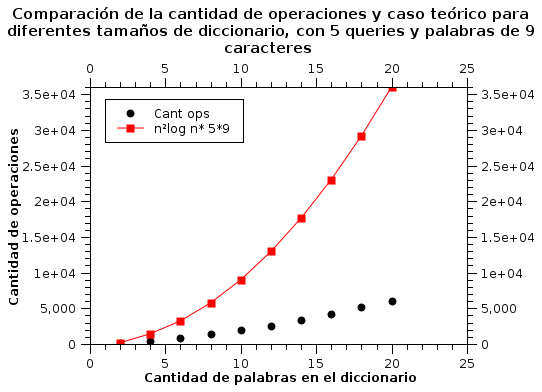
\includegraphics[scale=0.70]{graficos/2-3.png} \\
\scriptsize{\textsf{\textbf{Gr\'afico 2.3}}}  \\
\end{center}

Puede verse que las diferentes variables afectan a la cantidad de operaciones de diferente manera. El número de queries es lo que menos variación produce, esto puede entenderse porque ese cambio sólo afecta a la cantidad de veces que se aplica la función search, el diccionario sólo se construye una vez y se usa para todas las queries de la misma manera, por lo tanto su influencia es mínima y por ende no hay demasiados cambios. Es por esto que tampoco nos detuvimos a evaluar detenidamente la existencia de un peor caso que provoque un aumento desmedido de la cantidad de operaciones; la generación del diccionario es básicamente estándar y no varía mucho de acuerdo a las palabras en sí, tan solo a la cantidad de ellas y a su longitud; una query que pida palabras que están muy separadas una de la otra causaría una mayor cantidad de operaciones que dos adyacentes, pero como acabamos de demostrar las queries no afectan en sobremanera la cantidad de operaciones totales sino que son una parte bastante menor de éstas, por lo tanto, consideramos que evaluar un peor caso de esta manera no arrojaría resultados tan contundentes como para demostrar que éste es efectivamente un peor caso ya que la diferencia en cantidad de operaciones será relativamente menor.\\

Con respecto a variar la longitud máxima, se puede observar un cambio apreciable, ya que variar esto implica que cada comparación que se hace cuesta más; pero el mayor cambio se produce cuando se varía la cantidad de palabras, puede observarse que dado un número bajo de las mismas, aún cuando mantengamos las queries y la longitud alta la cantidad de operaciones es bajísima, y ésta crece rápidamente, esto puede explicarse porque la complejidad es cuadrática sobre las palabras pero sólo lineal sobre las queries y la longitud, por lo tanto es de esperar este comportamiento

\newpage
\subsection{Casos de Prueba}

En este ejercicio para poder demostrar la correctitud ejecutamos casos que nosotros consideramos importantes verificar, ya que son aquellos que cubren situaciones especiales que se podrían dar en el algoritmo\\

Estos casos (los cuales se pueden en $pruebas.txt$) son:
\begin{itemize}
\item Un caso en el que se buscaba un camino de una palabra a si misma, esperando como resultado un 0

\begin{verbatim}
dip
lip
mad
max
maple
may
mil
mal
pad
pil
pip
pod
pop
sap
sip
slice
slick
spice
stick
stock
*
maple maple

\end{verbatim}

Esto demuestra que el BFS no se ejecuta cuando no es necesario, y además que se comporta bien con componentes aisladas del grafo (obviamente, si está aislada el query debe contener la misma palabra como origen y destino para ser válida)

\item Casos en el que una palabra puede llegar a la palabra final a través de múltiples caminos. En estos casos debíamos verificar que el camino elegido sea el mas corto efectivamente.

Usando el mismo diccionario que antes
\begin{verbatim}
*
may mil
\end{verbatim}

En este caso, por ejemplo, para llegar de $may$ a $mil$ tiene varios caminos para elegir, pero el ideal es el que pasa sólo por $mal$ (u otro que camino que le permita pasar por una palabra intermedia); esto demuestra que nuestro BFS efectivamente recorre por niveles.

\item Una buena prueba que hicimos, modificando el caso anterior fue la de una vez elegido un camino, modificar o agregar una palabra que forzaba que deba cambiar el resultado ya que la agregada facilitaba un camino mas corto.

Usando el mismo diccionario y las mismas palabras de origen y destino que en el ítem anterior, probamos sin la palabra $mal$ en el diccionario y el camino que nos daba era más largo puesto que debía pasar por $mad$, $pad$, $pod$, $pop$, $pip$, $pil$ para llegar a $mil$, esto demuestra que el relacionados funciona correctamente porque $may$ y $mil$ no están relacionadas ya que tienen al menos dos diferencias, y entonces no hay eje entre ellas y el BFS tiene que hacer un camino muy largo para encontrar la conexión entre las mismas 
\newpage
\item  Ejecutamos casos en el que todo el grafo formado era completo, y por ende cada query que se hiciera entre palabras diferentes debería dar exactamente 1
\begin{verbatim}
hola
fola
tola
nola
mola
rola
gola
yola
*
hola tola
rola mola
nola yola
yola yola
hola gola
gola tola
mola yola
\end{verbatim}

Esto demuestra que el algoritmo se comporta bien ante grafos completos, y que siempre elige el camino mínimo que resulta ser 1, puesto que se puede ir de cualquier nodo a cualquier otro.

\end{itemize}

\newpage
\section{Ejercicio 3}

\subsection{Archivos}

En la carpeta $3$-$ej$ se puede encontrar
\begin{itemize}
\item $3$-$ej.cpp$: Algoritmo que resuelve el problema
\item $timer.cpp$: Usado para contar la cantidad de operaciones
\item $rangen.cpp$: Generador de inputs al azar
\item $pruebas.txt$ Casos borde usados para demostrar la correctitud
\item $Makefile$

\end{itemize}


\subsection{Enunciado}

El equipo de Calabozos y Dragones (CyD) de la facultad está muy preocupado porque varios de sus miembros estarán
de viaje por motivos académicos el cuatrimestre que viene. Es por esto que desea mantenerlos comunicados para poder
seguir con el cronograma deseado de juegos. Para esto definió dos tecnologías de interconexión entre los jugadores: Cada
jugador tendrá un celular y algunos de ellos además contarán con la ultima tecnología conexión a internet.

Dos jugadores con conexión a internet pueden comunicarse entre sí no importa su localización. En cambio, dos
jugadores pueden comunicarse por celular sólo si la distancia entre ellos no excede un cierto $D$. El $D$ depende del abono
pagado por el grupo. Obviamente, entre más grande D, mas costoso es el abono. Además, por tratarse de un plan para
grupos grandes, todos los celulares son idénticos, o sea que el valor $D$ para cualquier comunicación por celular es el mismo.
La cantidad de jugadores con conexión a internet es un número fijo, independiente del abono contratado.

Su trabajo es determinar quiénes tendrán conexión a Internet para que el $D$ necesario sea mínimo, de manera que el
grupo pueda contratar el abono más barato. Debe haber por lo menos un camino de comunicación (directo o indirecto)
entre cualquier par de jugadores.

\subsection{Breve descripción del algoritmo}

En este ejercicio teníamos que resolver de qué manera distribuir los dispositivos con internet para poder lograr contratar el abono mas económico, es decir el que menos distancia para contacto de teléfonos necesite. Para esto lo que hicimos fue modelar el problema como un grafo y aplicarle al mismo algún algoritmo conocido.

El modelo es el siguiente, cada jugador tiene una posición en el mapa, por lo tanto, un jugador para nosotros es un nodo en el grafo. Un nodo tiene un eje con otro nodo si y solo si pueden conectarse entre si. Como en principio, todo jugador puede conectarse con cualquier otro jugador, tenemos un grafo completo y por lo tanto conexo. Este grafo, además de tener ejes y nodos posee pesos en los ejes. Los pesos son iguales a la función distancia entre un jugador y el otro. 

La idea de modelar el grafo de esta manera, es poder usar algún algoritmo que me busque un árbol generador mínimo dentro del grafo completo, dándole la posibilidad al algoritmo de que tome cualquier eje como alternativa a la red que me comunique a todos los jugadores (nodos) de la forma mas barata (porque es AG mínimo).

Dentro de los algoritmos que calculan un árbol generador mínimo, conocemos el algoritmo de Kruskal y el algoritmo de Prim. Si bien los dos algoritmos dan un árbol generador mínimo nosotros decidimos usar Prim debido a que tiene una implementación mas sencilla a nuestra forma de ver los algoritmos.

Finalmente para elegir entre quienes habrá conexión a internet tomaremos aquellas aristas que mayor peso tengan una vez tenidas las aristas del AGM.

Resumiendo, nuestro algoritmo se traduce a modelar primero el problema como un grafo, luego ejecutar el algoritmo de Prim, quitar tantas aristas pesadas del AGM como conexiones a internet posibles. Luego la arista mas pesada del AGM es la distancia D del problema.

Un pseudocódigo que cumpla con todo esto realizara lo siguiente:\\

\newpage
\nuevoAlgo{Algoritmo 3}{ConexionMasBarata($jugadores$ : $conj<jugador>$, $conecciones$ :
$Nat$) $\rightarrow$ $D$ : $Nat$. Devuelve la Distancia D ya definida en el enunciado del problema}
\\

\begin{tabular}{rp{17cm}}
1: & ConexionMasBarata($jugadores$ : $conj<jugador>$, $conecciones$ : $Nat$)\{\vspace{0,1cm} \\  
2: & \hspace{0,5cm}   distancias : matriz$<$float$>$ $\gets$ Vacia \vspace{0,1cm} \\ 
3: & \hspace{0,5cm}   marcados : vector$<$bool$>$ $\gets$ todos en false y longitud == $\#$(jugadores)\vspace{0,1cm} \\ 
4: & \hspace{0,5cm}   $\forall$ i,j $\in$ jugadores \{\vspace{0,1cm} \\ 
5: & \hspace{1cm}	    distancias[i][j] $\gets$ calcularDistancia(i,j)\vspace{0,1cm} \\ 
6: & \hspace{0,5cm}	  \}\vspace{0,1cm} \\ 
7: & \hspace{0,5cm}	  marcados[0] $\gets$ true\vspace{0,1cm} \\ 
8: & \hspace{0,5cm}	  candidatos : $colaDePrioridad<ejes> \gets$ Vacia\vspace{0,1cm} \\ 
9: & \hspace{0,5cm}	  candidatos.push(ejesIncidentesA($jugadores_0$))\vspace{0,1cm} \\ 
10: & \hspace{0,5cm}	  AGM : $vector <ejes>$ $\gets$ Prim(jugadores, candidatos, distancias,
marcados)\vspace{0,1cm} \\ 
11: & \hspace{0,5cm}   AGM.OrdenarDeMayorAMenor()\vspace{0,1cm} \\ 
12: & \hspace{0,5cm}  devolver AGM[conecciones-1]\vspace{0,1cm} \\ 
13: & \}\\ \vspace{0,1cm} \\ 
\end{tabular}

\nuevoAlgo{Algoritmo 4}{Prim($jugadores$ : conj$<$jugador$>$, $candidatos$ :
colaDePrioridad$<$ejes$>$, distancias : matriz$<$float$>$, marcados : vector$<$bool$>$)
$\rightarrow$ $res$ : vector$<$ejes$>$. Devuelve un vector de ejes con su peso que forman un AGM.}
\\

\begin{tabular}{rp{17cm}}
1: & Prim($jugadores$ : conj$<$jugador$>$, candidatos : colaDePrioridad$<$ejes$>$, distancias :
matriz$<$float$>$)\{\vspace{0,1cm} \\ 
2: & \hspace{0,5cm}   aristasFaltantes : Nat $\gets$ $\#$(jugadores) - 1 \vspace{0,1cm} \\ 
3: & \hspace{0,5cm}   res : $vector<ejes>$ $\gets$ Vacio\vspace{0,1cm} \\ 
4: & \hspace{0,5cm}   $\mientras$ aristasFaltantes $>$ 0 \{\vspace{0,1cm} \\ 
5: & \hspace{1cm}       minimo : eje $\gets$ candidatos.top()\vspace{0,1cm} \\ 
6: & \hspace{1cm}       $\mientras$ estaMarcadoAmbosNodos(minimo, marcados)\vspace{0,1cm} \\ 
7: & \hspace{1,5cm}       candidatos.pop()\vspace{0,1cm} \\ 
8: & \hspace{1,5cm}       minimo = candidatos.top()\vspace{0,1cm} \\ 
9: & \hspace{1cm}       \}\vspace{0,1cm} \\ 
10: & \hspace{1cm}       nodo : jugador $\gets$ noMarcado(nodos(minimo))\vspace{0,1cm} \\ 
11: & \hspace{1cm}       marcados[nodo] $\gets$ true\vspace{0,1cm} \\                       
12: & \hspace{1cm}       res.push(minimo)\vspace{0,1cm} \\ 
13: & \hspace{1cm}       agregarAristas(nodo, candidatos)\vspace{0,1cm} \\ 
14: & \hspace{1cm}       aristasFaltantes $\gets$ aristasFaltantes - 1\vspace{0,1cm} \\ 
15: & \hspace{0,5cm}    \}\vspace{0,1cm} \\ 
16: & \hspace{0,5cm}    $\devolver$ res \vspace{0,1cm} \\ 
17: & \}\\ \vspace{0,1cm} \\ 
\end{tabular}



\subsection{Correctitud}

En esta sección del problema nos preocuparemos de explicar porque el algoritmo propuesto por nosotros se encarga de otorgar una solución del enunciado.

Como la solución del problema consta de dos partes, nos encargaremos de explicar porque ambas son correctas. Primero pasaremos a explicar porque el modelo es adecuado.\\

El ejercicio pide que demos una forma de conectar a todos los jugadores (no mediante un grafo completo, sino que formando una red de comunicación) y darle a ellos una posible forma de conectarse, mediante internet o mediante celulares, de tal forma que la conexión mas lejana utilizando celular sea la mínima posible. Para nosotros los jugadores serán nodos y modelamos un grafo completo, es decir, todos los jugadores conectados entre si, ya que en un principio cualquier jugador (nodo) podría estar conectado con cualquier otro jugador (nodo). Como quiero obtener las distancias mas convenientes vamos a agregarle a los ejes como peso, la distancia entre cada par de nodos. La idea de modelarlo así es obtener luego un AGM que cumple con la solución\\

Luego de explicar el modelo, vamos a explicar porque obtener un AGM de este grafo es una solución.

Tenemos que armar una red de comunicación entre los jugadores. Como los jugadores son nodos, es lo mismo que pedir un árbol ya que estarían formando una cadena de comunicación que mantiene a todos los jugadores (nodos) unidos. Es importante darle al algoritmo aplicado la posibilidad de que elija cualquier conexión entre todo par de nodos, es por esto que en un principio el grafo es completo, para que pueda elegir que nodos relacionar mediante un eje. Luego la solución es un árbol.

Ahora veamos que el árbol pedido es un subgafo del grafo original (el grafo completo). Luego la solución es un AG.

Por ultimo, las conexiones entre los nodos deben $"intentar"$ ser los mínimos. Utilizamos la palabra intentar porque si bien la idea en un principio es colocar todos los ejes mas chicos, puede que alguno de esos forme ciclo, rompiendo la propiedad de que la solución sea una red. Luego si quiero obtener los ejes mas livianos del grafo, evitando aquellos casos donde el eje forma ciclo, entonces lo que busco es un AGM del grafo completo formado por los jugadores y de pesos iguales a las distancias entre ellos.\\

El único detalle que falta aclarar es que una vez que tenemos el AGM, tenemos $x$ conexiones que podemos hacer $"gratis"$ debido a que unimos dos jugadores (nodos) mediante una conexión de internet. Por lo tanto, de todos los ejes ordenados de mayor a menor según su peso, voy a pedir el peso del $x+1$-esimo eje ya que a los anteriores a este les daremos conexión de internet. Le damos tecnología de internet a los ejes mas pesados ya que de esta forma minimizamos la conexión por celular mas lejana.

Finalmente veamos que nuestro pseudocódigo se encarga de hacer todo lo descrito: modela el grafo obteniendo la matriz de distancias entre cada par de nodo, ejecuta el algoritmo de Prim que pasaremos a contar su correctitud mas adelante y luego obtiene el peso del eje $x+1$-esimo luego de ordenarlos por peso de mayor a menor.

\subsubsection*{Correctitud de Prim}

Tomamos un nodo, lo marcamos y colocamos como posibles ejes a poner en el vector res a sus adyacentes. Tomamos el mínimo de estos ejes. Luego de elegir este eje, marcamos el nodo incidente al eje que no estaba marcado anteriormente y colocamos sus ejes adyacentes como posible candidato exceptuando aquellos ejes que tengan ambos nodos incidentes marcados. Tomaremos de todo el conjunto de candidatos el mínimo nuevamente y exceptuando los ejes cuyos nodos están ambos marcados. Repetiremos esto hasta tener todos los nodos marcados.

Como nunca toma ejes cuyos nodos están ambos marcados, evito que se cree un ciclo. Además como en cada paso marco un nodo que no fue anteriormente marcado y empezamos con un nodo marcado, en la iteraron final, es decir, la $n - 1$ con $n = \#$(jugadores), tenemos un AGM porque no tiene ciclos, posee todos los nodos del grafo, y es mínimo debido que siempre tomamos el mínimo nodo posible.



\subsection{Complejidad}

Para analizar la complejidad de nuestro algoritmo analizaremos el pseudocódigo paso a paso. Lo separaremos en dos secciones, la complejidad del algoritmo de Prim y de la función general que resuelve el problema

\subsubsection*{Análisis de la complejidad de Prim}

% \begin{tabular}{rp{15cm}}
En las instrucciones 2 y 3 hacemos operaciones constantes. Pedir la cantidad de jugadores es dato del problema y crear un vector vacío es constante de acuerdo a la documentación de la standard library de $C++$. Luego se inicia un ciclo va a terminar recorriendo todos los ejes del grafo para asegurarse de generar el AGM correcto. 
Si bien la iteración es sobre el número de aristas faltantes y por ende se puede pensar que lo va a hacer $n-1$ veces, debemos recalcar que el algoritmo va a recorrer todas las aristas y por ende la cantidad de veces que se itera es $m$. Antes de entrar al ciclo se pushean en el heap todos los ejes que tienen como extremo al primer nodo; dentro del mismo, le pedimos que nos dé el eje de mínimo peso de la cola. 
Esta instrucción usa la función $top()$\footnotemark \footnotetext[9]{\url{http://www.cplusplus.com/reference/stl/priority\_queue/top/}} del contenedor priority\_queue. De acuerdo a la documentación, esta función tiene un costo constante. Verificamos que el segundo extremo del eje no esté marcado (como es mirar en un array, esto es constante), si lo está, lo descartamos con la función $pop()$\footnotemark \footnotetext[10]{\url{http://www.cplusplus.com/reference/stl/priority\_queue/pop/}} del contenedor priority\_queue que según la documentación tiene costo logarítmico en la cantidad de elementos de la cola, tal como lo muestran las filas 6-9; si sirve, lo agregamos al AGM en tiempo constante y lo popeamos, seguidamente agregamos todas las aristas que están conectadas con ese nodo (o sea, por cada nodo que agregamos al AGM recorremos todos los otros para ver si están marcados o no). 
En resumen, para cada nodo recorremos todos sus adyacentes (o sea, todos los otros, porque es completo), y para cada eje lo agregamos a un heap en tiempo logarítmico y después o bien lo descartamos o bien lo agregamos al AGM, popeandolo del heap nuevamente en tiempo logarítmico, por ende, la complejidad de Prim es $O(n^{2} * log(n))$  .\\





Recapitulando vimos que este algoritmo ejecuta $n$ veces un ciclo que contiene dentro otro ciclo que se ejecuta a lo sumo $n$ veces en peor caso. Dentro del segundo ciclo, ejecutamos una instrucción que cuesta $log(n)$. Además ejecuto dentro del primer ciclo otro ciclo pequeño que, en peor caso, ejecuta $n$ veces una instrucción de costo logarítmico en $n$. Dando la siguiente formula:

\begin{center}
$O(n * (n * log(n) + n * log(n))) = O(n * (2n * log(n))) = O(2n^2 * log(n)) \in O(n^2 * log(n))$
\end{center}



\subsubsection*{Análisis de la complejidad de ConexionMasBarata}


\begin{tabular}{rp{15cm}}
2-3: & Inicializamos una matriz y un vector. Los constructores de ambos contenedores son constantes de acuerdo a la documentación de la biblioteca de $C++$\\
4-6: & En cada celda de la matriz realizamos la calculamos la distancia entre nodos utilizando la formula de la distancia entre puntos. Ejecutar esta cuenta tiene costo constante para el análisis de la complejidad utilizando el modelo universal. Pero como se calcula esto por cada celda de la matriz cuyo tamaño es de NxN, este conjunto de instrucciones tiene un costo total de $O(n*n)$\\
7-8: & En estas instrucciones realizo operaciones constantes, cabe destacar que inicializar una cola de prioridad vacía tiene costo constante, de acuerdo a lo dicho en la documentación de $C++$\\
9: & Utilizo la función $push()$\footnotemark  del contenedor de priority\_queue de $C++$ $n$ veces porque el grafo es completo, por lo tanto un nodo tiene $n-1$ ejes.\\
10: & Llamo a Prim, anteriormente dijimos que tenia costo $O(n^2 * log(n))$\\
11: & Hacemos la llamada a $sort()$\footnotemark función que ordenará nuestro vector de mayor a menor con costo, de peor caso de $n^2$\\
12: & Indexamos en el vector, esto cuesta $O(1)$\\
\end{tabular}

\footnotetext[11]{\url{http://www.cplusplus.com/reference/stl/priority\_queue/push/}}
\footnotetext[12]{\url{http://www.cplusplus.com/reference/algorithm/sort/}}
\vspace{0,5cm}



Finalmente obtenemos que nuestro algoritmo cuesta en total:

\begin{center}
$O(n^2) + O(n^2 * log(n)) + O(n^2) \in O(n^2 * log(n))$
\end{center}

Podemos observar que $O(n^2 * log(n)) < O(n^3)$ debido a que $O(log(n)) < O(n)$. Luego cumplimos con la cota pedida por el ejercicio.




\subsection{Tablas y Gráficos}

Para el estudio de este ejercicio, nos valimos de dos archivos auxiliares, $timer.cpp$ y $rangen.cpp$, éste último se encarga de generar una entrada de números aleatorios para una cantidad de jugadores y conexiones pedida. Para el primer archivo, éste consta del mismo código que el algoritmo principal, pero modificado para sumar la cantidad de operaciones que se efectúan y luego devolverlo al final del mismo.

A simple vista, para considerar cómo la entrada afecta al tiempo que toma resolver el algoritmo se puede pensar que se tiene dos variables, una que sería la cantidad de jugadores y otra que sería la cantidad de conexiones de internet disponibles para asignar. Nuestro primer objetivo es demostrar que la cantidad de conexiones afecta muy poco en la resolución. Se puede ver en el código que esa variable sólo la usamos en dos instancias; una al principio, cuando filtramos los casos bordes que serían cuando la cantidad de conexiones es mayor o igual a la cantidad de jugadores y por ende eso hace inútil el cálculo del AGM ya que la distancia a comprar va a ser siempre cero; y luego al final, cuando con el AGM calculado decidimos cuántas ramas descartar hasta dar con la solución. Se puede ver que es un acceso a un arreglo usando como índice éste parámetro, por lo tanto no va a cambiar en nada que haya muchas o pocas conexiones (siempre y cuando no se entre al primer filtro, por supuesto). Es por esto que primero presentamos un estudio sobre la cantidad de operaciones contadas con $timer.cpp$ variando la cantidad de conexiones y dejando fijo el número de jugadores ($n = 100$)


\begin{center}
\begin{tabular}{|c|c|}
\hline
Cantidad de conexiones de internet & Cantidad experimental de operaciones para 100 jugadores\\
\hline
1	 & 50,445\\
\hline
3	 & 51,303\\
\hline
5	 & 51,095\\
\hline
10	 & 51,291\\
\hline
20	 & 50,776\\
\hline
30	 & 51,790\\
\hline
40	 & 50,585\\
\hline
50	 & 50,821\\
\hline
60	 & 51,880\\
\hline
70	 & 50,647\\
\hline
80	 & 50,725\\
\hline
90	 & 50,832\\
\hline
99	 & 51,275\\
\hline
\end{tabular}
\end{center} \vspace{0,15cm}



\begin{center}
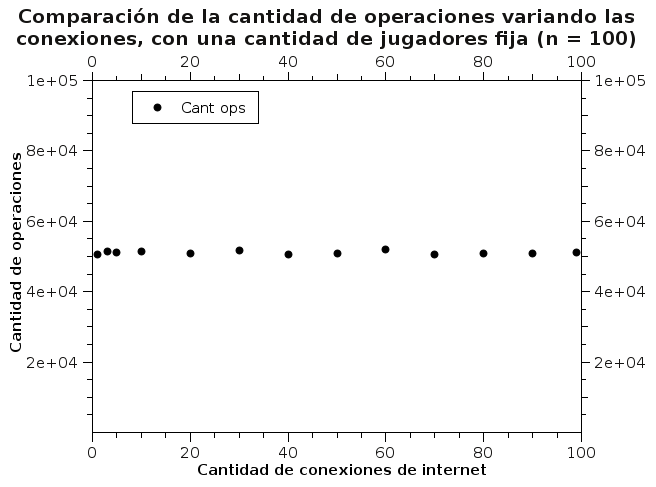
\includegraphics[scale=0.60]{graficos/3-1.png} \\
\scriptsize{\textsf{\textbf{Gr\'afico 3.1}}}  \\
\end{center}

Se puede observar tanto en el gráfico como en la tabla que lo que propusimos nosotros es correcto, la cantidad de operaciones no se ve afectada por la cantidad de conexiones, ya que dado un número de jugadores, siempre y cuando éstas no entren en un caso borde, el número de operaciones se mantiene prácticamente constante. Es por esto que para el resto del análisis podemos descartar la cantidad de conexiones y simplemente decir que vamos a elegir un número que haga que no caiga en un caso borde.\\

Consideramos que no existe un input en este problema que sea un evidente peor caso, ya que nuestro algoritmo se comporta de manera muy similar para todos. Es decir, para un determinado número de jugadores (ya explicamos por qué la cantidad de conexiones no influye), el AGM se va a generar de la misma manera, ya que todos los ejes van a ser pusheados y descartados o aceptados, pueden cambiar los distancias pero en sí el no hay valores especiales que afecten la complejidad de nuestros cálculos, por lo tanto descartamos la existencia de un caso especial que debamos considerar que nos cause un peor caso muy notable.\\

Por lo tanto, presentamos a continuación el estudio hecho sobre la cantidad de operaciones resultantes para diferentes cantidades de jugadores, y el gráfico obtenido

\begin{center}
\begin{tabular}{|c|c|c|}
\hline
Cantidad de jugadores & Cantidad experimental de operaciones & Caso Teórico: $4 * n^{2} log (n)$\\
\hline
10	 & 175	 & 800\\
\hline
100	 & 50,552 & 	120,000\\
\hline
200 & 	213,267	 & 480,000\\
\hline
300	 & 490,487 & 	1,080,000\\
\hline
400	 & 894,285	 & 2,560,000\\
\hline
500 & 	1,421,150 & 	4,000,000\\
\hline
600	 & 2,074,240	 & 5,760,000\\
\hline
700 & 	2,858,021 & 	7,840,000\\
\hline
800	 & 3,771,169	 & 10,240,000\\
\hline
900	 & 4,821,477 & 	12,960,000\\
\hline
1,000	 & 5,990,652 & 	16,000,000\\
\hline
1,100 & 	7,309,868 & 	19,360,000\\
\hline
1,200	 & 8,766,232 & 	23,040,000\\
\hline
\end{tabular}
\end{center} \vspace{0,15cm}



\begin{center}
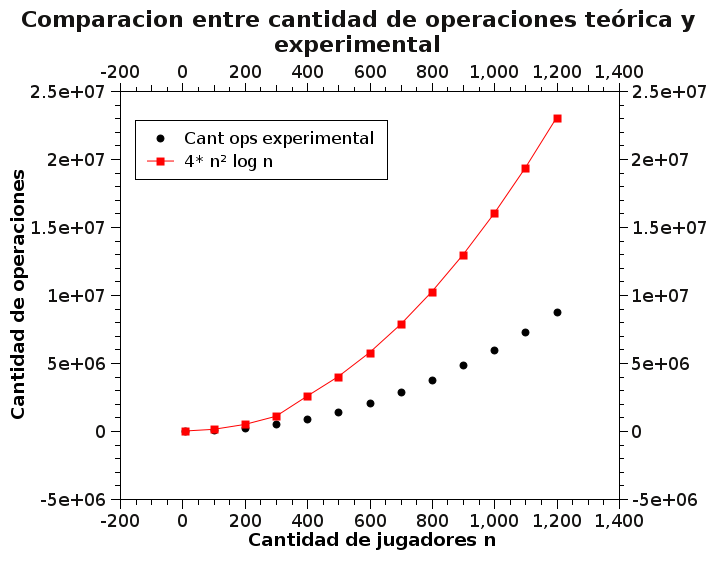
\includegraphics[scale=0.60]{graficos/3-2.png} \\
\scriptsize{\textsf{\textbf{Gr\'afico 3.2}}}  \\
\end{center}

Se puede observar que la cantidad de operaciones se mantiene por debajo de la curva $k* n^{2} *log (n)$, siendo $k = 4$.

\newpage
\subsection{Casos de Prueba}

En este ejercicio evaluamos distintas series de pruebas que nos de como resultado final el valor esperado para asi demostrar la correctitud del algoritmo
En el caso en que debíamos asignar en primer lugar cantidad de usuarios y de móviles con internet que poseían, y luego asignar coordenadas, nos permitimos probar múltiples casos jugando con los diferentes tipos de datos. Estos casos de prueba se pueden encontrar en el archivo $pruebas.txt$.

\begin{itemize}
\item Probamos con 2 personas en la que una tenga internet y la otra no, este caso debía dar la distancia entre sus coordenadas ya que es la única comunicación posible. También este caso debe ser así cuando hay 2 personas sin dispositivos con internet disponibles.
\begin{verbatim}
1 2
232 210
123 12

0 2
10 0
20 41
\end{verbatim}

Esto demuestra que en el caso de haber sólo dos personas el algoritmo genera el AGM que resulta ser el único camino posible y de ahí no resta caminos (si hay una sola internet, pregunta por el $[0]$ de la misma manera en el AGM) si no puede hacerlo

\item Probamos con 2 personas pero esta vez con ambas con internet, este caso al tener una libre comunicación el resultado debe ser una distancia de 0.

\begin{verbatim}
2 2
100 23
25 40
\end{verbatim}

Esto demuestra que en el caso borde de haber la misma cantidad de conexiones que de jugadores, se entra en la guarda antes de generar todo el árbol y se evita todo el cálculo ya que se conoce de antemano el resultado que es $0.00$

\item Luego ya con una cantidad razonable de usuarios y dispositivos con internet, probamos con ubicar a todos los jugadores en el mismo lugar.

\begin{verbatim}
2 5
20 20
20 20
20 20
20 20
20 20
\end{verbatim}
Esto demuestra que el AGM toma bien las distancias porque éstas terminan siendo 0, y aún cuando se genere todo el árbol (ya la cantidad de conexiones es menor que la de jugadores y por ende se necesita hacer todo el algoritmo), las aristas del AGM quedan con peso 0 y se devuelve el resultado correcto en el algoritmo.
\end{itemize}


\end{document}